\documentclass[final]{beamer}

\usepackage[T1]{fontenc}
\usepackage{lmodern}
\usepackage[orientation=portrait,size=a0,scale=1.0]{beamerposter}
\usetheme{gemini}
\usecolortheme{nott}
\usepackage{graphicx}
\usepackage{booktabs}
\usepackage{tikz}
\usepackage{pgfplots}
\pgfplotsset{compat=1.14}
\usepackage{anyfontsize}
\usepackage{xcolor}
\usepackage{microtype}

% Custom colours
\definecolor{afgreen}{RGB}{45, 106, 79}
\definecolor{edgered}{RGB}{230, 57, 70}
\definecolor{steelblue}{RGB}{69, 123, 157}
\definecolor{warnorange}{RGB}{230, 100, 20}

% Layout
\newlength{\sepwidth}
\newlength{\colwidth}
\setlength{\sepwidth}{0.018\paperwidth}
\setlength{\colwidth}{0.306\paperwidth}
\newcommand{\separatorcolumn}{\begin{column}{\sepwidth}\end{column}}

% -----------------------------------------------------------------------
\title{Does Federated Learning Need a Crowd?\\[0.3ex]
{\large Client Count, Not Heterogeneity, Explains FedAvg's Failure on Real Edge Hardware}}

\author{Daniel Akhabue\inst{1,2} \and David Akhabue\inst{2}}

\institute[shortinst]{%
  \inst{1}~Qucoon, Nigeria \quad
  \inst{2}~Machine Learning Collective (MLC)\\[0.4ex]
  \href{mailto:danakhabue@gmail.com}{danakhabue@gmail.com} \quad
  \href{mailto:daviesakhs009@gmail.com}{daviesakhs009@gmail.com}}

\footercontent{%
  \href{mailto:danakhabue@gmail.com}{danakhabue@gmail.com}
  \hfill
  Deep Learning Indaba 2026 -- RIAD Poster Session
  \hfill
  Research in Africa Days}

\logoleft{\hspace{5cm}
\includegraphics[height=10cm]{logos/logo.png}}
\logoright{
\includegraphics[height=10cm]{logos/logo.png}}
% -----------------------------------------------------------------------

\begin{document}
\begin{frame}[t]
\begin{columns}[t]
\separatorcolumn

%% =====================================================================
%% COLUMN 1
%% =====================================================================
\begin{column}{\colwidth}

  \begin{block}{Abstract}
    \small
    Federated learning is routinely presented as a strictly beneficial
    alternative to centralized or local-only training on edge devices,
    since it preserves data sovereignty and minimises communication while
    supposedly matching or exceeding centralized accuracy. We test this
    assumption directly on real, physically heterogeneous edge hardware
    -- an ARM64 Raspberry Pi~4 and an x86\_64 gateway machine --
    federating a compact anomaly detection model across them with the
    standard FedAvg algorithm. Contrary to the common assumption, we find
    that naive FedAvg \textbf{consistently and substantially underperforms}
    both local-only training on the stronger device and simple centralized
    pooling, a result that holds across three independent random seeds and
    \textit{worsens} the longer training continues. We then isolate the
    cause through a controlled experiment holding the real ARM64-vs-x86\_64
    data heterogeneity fixed while varying only client count. Federated
    accuracy improves monotonically and variance shrinks sharply as client
    count rises from 2 to 8, even though the underlying heterogeneity never
    changes. \textbf{Client count, not heterogeneity, explains the failure.}
    This carries direct practical weight for small edge fleets where
    federated learning is often adopted by default without first verifying
    that minimal-client federation will not actively underperform simpler
    alternatives.
  \end{block}

  \begin{block}{Introduction}
    \small
    Edge devices intended for on-device anomaly detection -- perimeter
    sensors, surveillance cameras, gateway nodes, drone payloads -- must
    learn collaboratively while respecting three binding constraints:
    \vspace{0.2em}
    \begin{itemize}\setlength\itemsep{0.15em}
      \item \textbf{Compute scarcity:} ARM-class CPUs, 4--8\,GB RAM;
            large models are infeasible.
      \item \textbf{Bandwidth scarcity:} 2G/EDGE or intermittent links;
            streaming raw telemetry to a server is impractical.
      \item \textbf{Data sovereignty:} raw sensor data must not leave
            the device for regulatory or trust reasons.
    \end{itemize}
    \vspace{0.2em}
    FedAvg~\cite{fedavg} satisfies all three by exchanging only model
    weight updates. Prior work demonstrates this is feasible at moderate-to-large
    fleet size. What is comparatively under-examined is whether this benefit
    holds in the \textit{minimal-client} regime -- two or three physical
    devices -- the realistic starting point for most edge deployments before
    they scale, and the scenario this work investigates on real hardware.
  \end{block}

  \begin{block}{Related Work}
    \small
    FL for edge/IoT anomaly detection is well-established.
    \textbf{FedIoT}~\cite{fediot} demonstrates FedAvg-based attack
    detection on real Raspberry Pi fleets with affordable training cost.
    \textbf{TinyFL} achieves F1$\approx$97\% on ESP32 industrial nodes
    over constrained networks~\cite{tinyfl}. A federated LSTM autoencoder
    on the \textbf{Marconi100 supercomputer} improves F1 from 0.39 to 0.87
    across 100 compute nodes~\cite{marconi}. A \textbf{Pi-based smart-grid
    testbed} benchmarks FL feasibility via CPU/memory/power/bandwidth across
    seven models~\cite{smartgrid}.

    \vspace{0.2em}
    \textbf{What is missing:} none of these works explicitly isolate client
    count as a variable while holding genuine, hardware-derived heterogeneity
    fixed, nor report the specific failure mode we document here -- that
    naive FedAvg can underperform both alternatives with only two or three
    real clients, regardless of how heterogeneous those clients are.
  \end{block}

  \begin{alertblock}{Research Question}
    \small\centering
    \textit{Does FedAvg provide an accuracy benefit over local-only and
    centralized training when the federation has only two or three real
    devices? And if it underperforms, is the cause data heterogeneity
    between those devices, or the small number of participants itself,
    independent of heterogeneity?}
  \end{alertblock}

  \begin{block}{Method}
    \small
    \textbf{Model:} MLP ($11{\to}32{\to}16{\to}2$, ReLU), $\approx$700
    params, $<$10\,KB, $<$1\,ms/sample inference.

    \vspace{0.15em}
    \textbf{Devices:} Raspberry Pi~4 (ARM64) and an x86\_64 gateway --
    different ISA, thermal behavior, and frequency scaling produce
    \textit{naturally} non-IID telemetry without synthetic partitioning.

    \vspace{0.15em}
    \begin{figure}
      \centering
      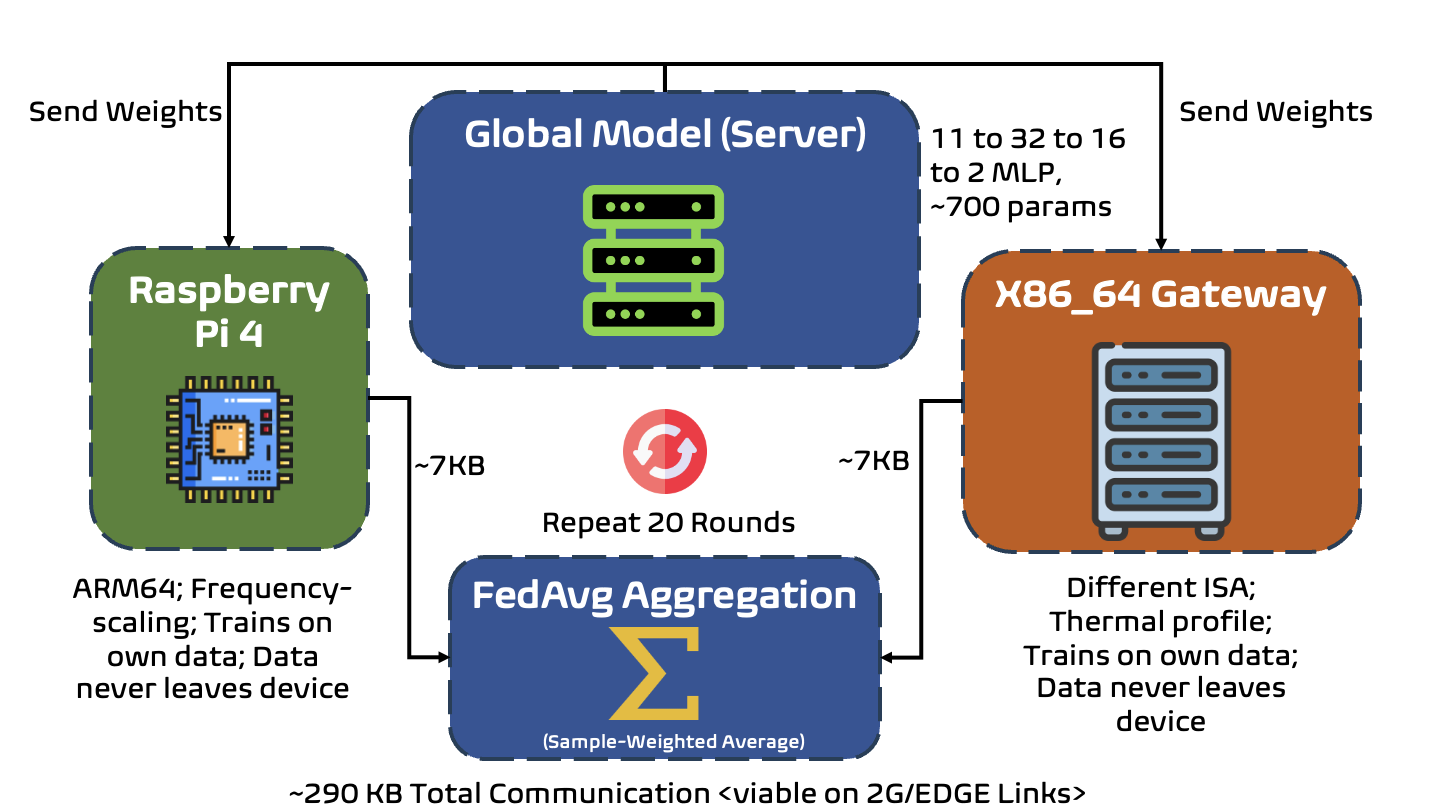
\includegraphics[width=0.95\colwidth]{results/architecture_diagram.png}
    \end{figure}
    \vspace{-0.2em}
    {\footnotesize Fig.\,1. Federation architecture: only weight vectors
    ($\approx$7\,KB/round) are transmitted; raw data stays on-device.}

    \vspace{0.15em}
    \textbf{Matched budget:} all three conditions receive an identical
    100-iteration budget (20 rounds $\times$ 5 epochs), eliminating
    training-time as a confound.

    \textbf{Methods:} local-only (no communication), centralized
    (data pooled), federated (FedAvg~\cite{fedavg}, 20 rounds).

    \textbf{Protocol:} 3 independent random seeds; mean and std reported.
  \end{block}

\end{column}
\separatorcolumn

%% =====================================================================
%% COLUMN 2
%% =====================================================================
\begin{column}{\colwidth}

  \begin{block}{Dataset}
    \small
    Telemetry logged at 1\,Hz from both real devices over $\approx$4\,h
    each; real \texttt{stress-ng} anomalies injected identically on
    \textbf{both} (CPU spikes, memory pressure, I/O storms, disk thrash,
    cache pressure). 11 features: CPU\%, freq, load avg (1m/5m), mem\%,
    mem\,MB, swap\%, disk R/W, net sent/recv.

    \vspace{0.3em}
    \begin{table}
      \centering\small
      \begin{tabular}{l r r}
        \toprule
        \textbf{Device} & \textbf{Rows} & \textbf{Anomaly\%} \\
        \midrule
        Pi~4 (ARM64)      & 14,354 & 23.1\% \\
        Gateway (x86\_64) & 14,313 & 23.2\% \\
        \midrule
        Combined          & 28,667 & 23.2\% \\
        \bottomrule
      \end{tabular}
    \end{table}
    {\footnotesize Near-identical anomaly rates confirm the collection
    schedule executed consistently on both platforms.}
  \end{block}

  \begin{block}{Experiments}
    \small
    Three experiments establish, test, and explain the central finding:

    \vspace{0.3em}
    \begin{table}
      \centering\small
      \begin{tabular}{p{0.28\colwidth} p{0.28\colwidth} p{0.28\colwidth}}
        \toprule
        \textbf{Exp.\,1} & \textbf{Exp.\,2} & \textbf{Exp.\,3} \\
        Real-hardware & Client-count & Heterogeneity \\
        federation & isolation & sweep \\
        \midrule
        2 real clients & 2--8 clients & 10 simulated \\
        (Pi + gateway) & (sub-divided & clients \\
                       & real data) & \\
        3 seeds & 3 seeds & 5 seeds \\
        Establishes the & Isolates client & Reference at \\
        failure & count as cause & higher $K$ \\
        \bottomrule
      \end{tabular}
    \end{table}
  \end{block}

  \begin{alertblock}{Results: FedAvg Fails on 2 Real Clients}
    \small
    \begin{table}
      \centering\small
      \begin{tabular}{l c c c}
        \toprule
        \textbf{Setting} & \textbf{Seed 42} & \textbf{Seed 1} &
        \textbf{Seed 7} \\
        \midrule
        Pi local only     & 0.952 & 0.945 & 0.952 \\
        Gateway local     & 0.851 & 0.848 & 0.836 \\
        Centralized       & 0.895 & 0.893 & 0.890 \\
        \midrule
        \textbf{Federated}& \textbf{0.789} & \textbf{0.770} &
        \textbf{0.749} \\
        \bottomrule
      \end{tabular}
    \end{table}

    \vspace{0.2em}
    \begin{itemize}\setlength\itemsep{0.15em}
      \item Federation is \textbf{worst in every seed} by 0.10--0.14 F1
            points below centralized, despite an identical matched training
            budget.
      \item F1 peaks near round~5 ($\approx$0.83) then \textbf{degrades
            through round~20} ($\approx$0.75--0.79): more rounds actively
            hurt performance.
      \item Communication cost: 290\,KB total, 14.5\,KB/round (viable
            on 2G), but bandwidth savings do not offset the accuracy cost.
    \end{itemize}

    \vspace{0.2em}
    \begin{figure}
      \centering
      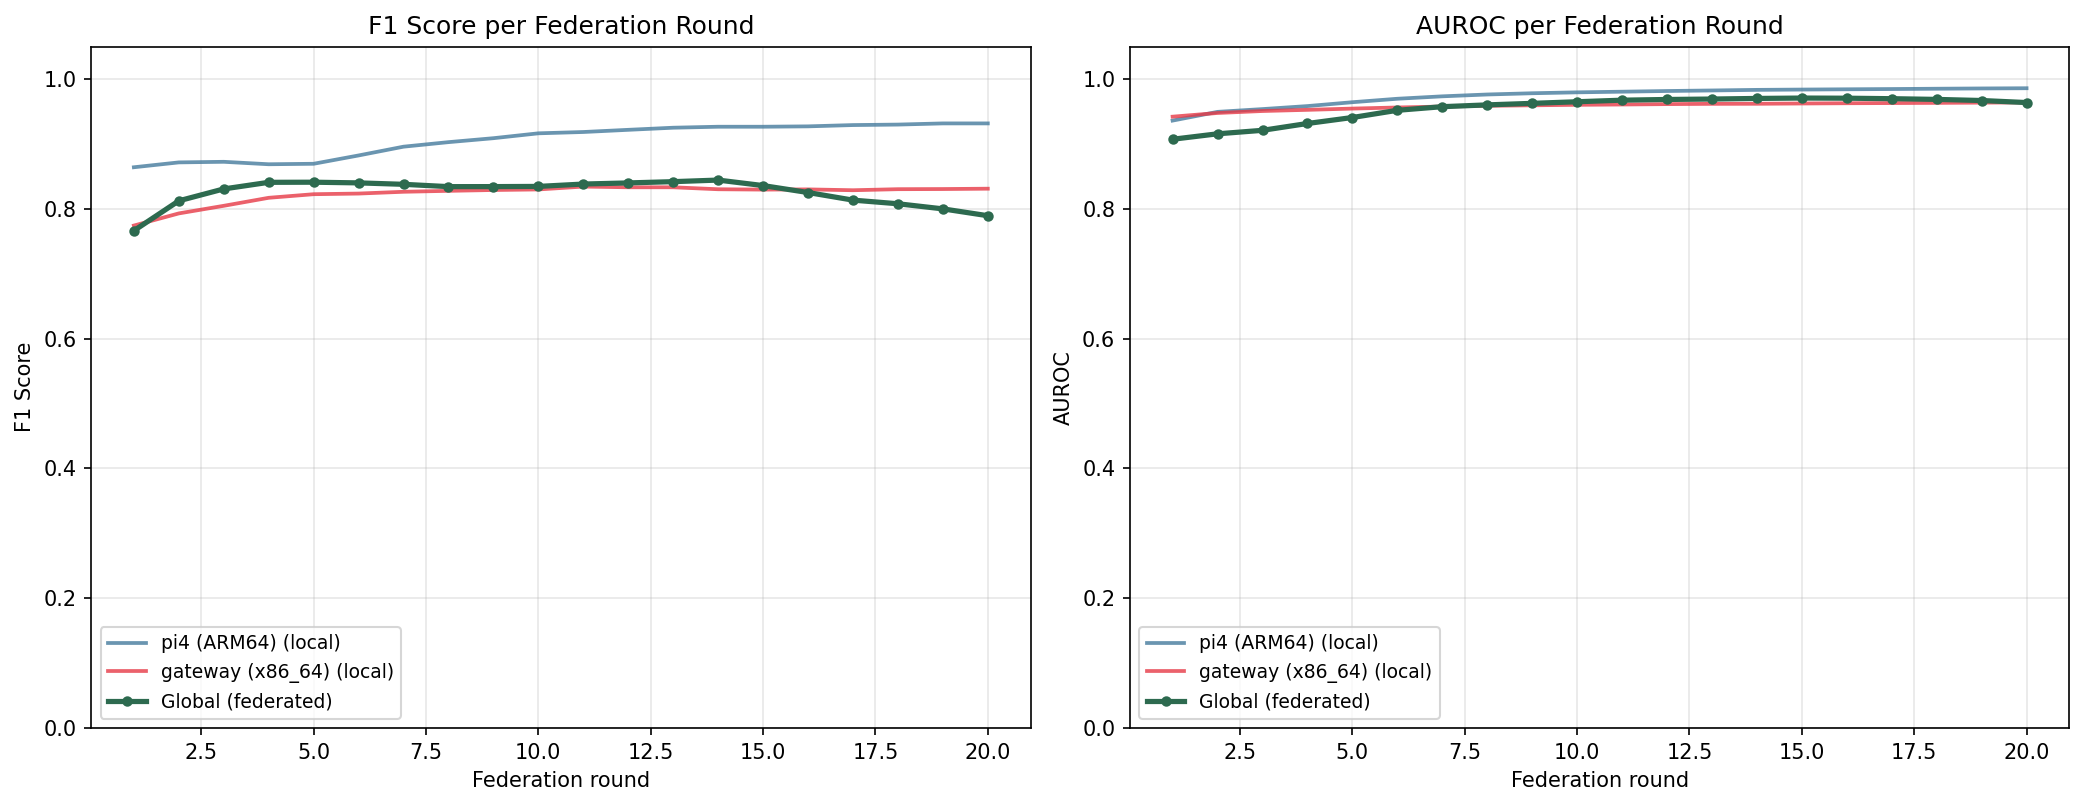
\includegraphics[width=0.95\colwidth]{results/convergence_plot.png}
    \end{figure}
    {\footnotesize Fig.\,2. Per-round F1/AUROC: federated model peaks early
    then degrades, while client models train independently.}
  \end{alertblock}

  \begin{block}{Real-Hardware Validation}
    \small
    The result is consistent and robust: across all three seeds the
    ordering is always Pi-local $>$ Centralized $>$ Gateway-local $>$
    Federated. The systematic round-by-round degradation (peak at round 5,
    decline to round 20) replicates across all seeds, ruling out a single
    unlucky initialization as the explanation and pointing to a structural
    property of FedAvg's averaging step with two clients.
  \end{block}

  \begin{alertblock}{Client-Count Isolation Study}
    \small
    To separate the contribution of data heterogeneity from client count,
    we split each real device's data into $k$ sub-clients ($k$=1--4),
    keeping Pi-derived and gateway-derived data strictly separated, so
    the genuine ARM64-vs-x86\_64 heterogeneity is \textbf{held constant}
    while only total client count changes (2, 4, 6, 8).

    \vspace{0.15em}
    \begin{figure}
      \centering
      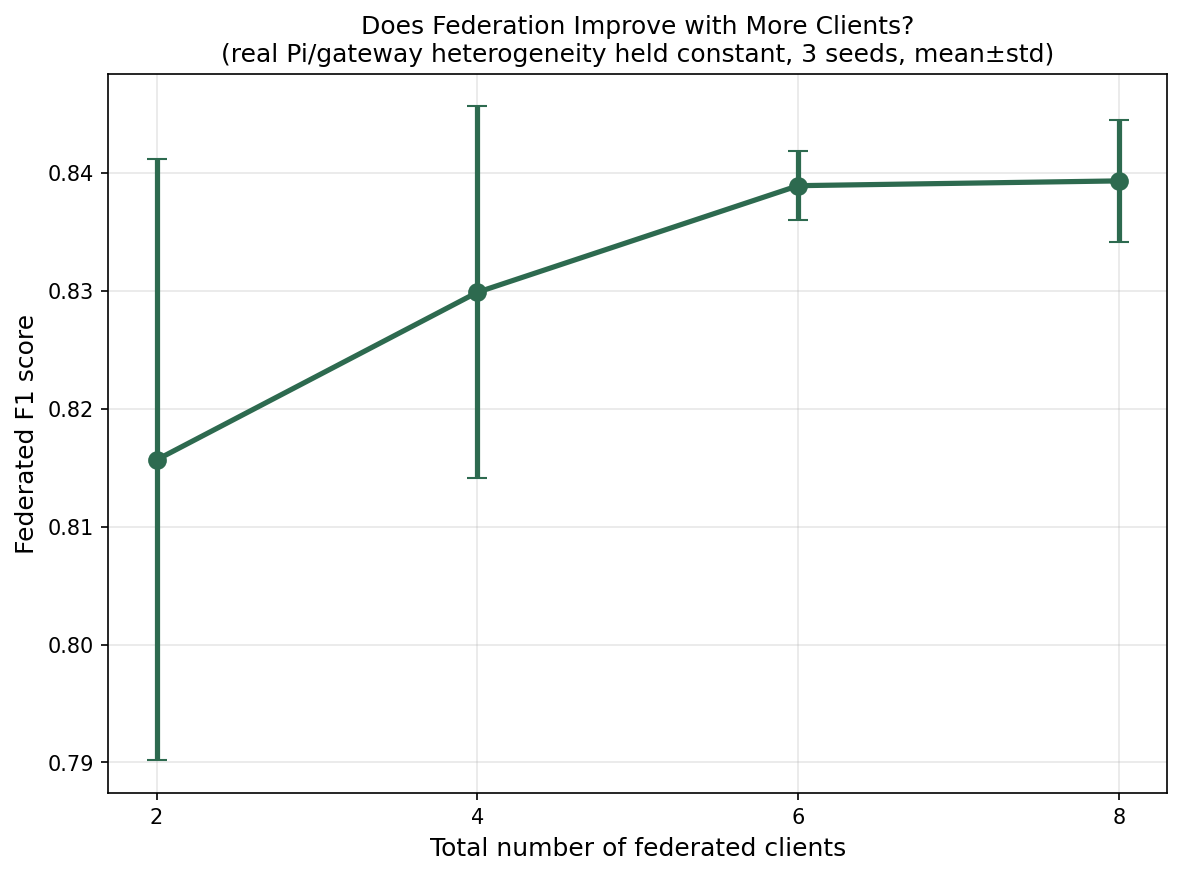
\includegraphics[width=0.85\colwidth]{results/client_count_isolation.png}
    \end{figure}
    \vspace{-0.3em}
    {\footnotesize Fig.\,3. Federated F1 vs.\ total client count, real
    heterogeneity fixed, 3 seeds, mean$\pm$std.}

    \vspace{0.15em}
    \begin{table}
      \centering\small
      \begin{tabular}{r r c c}
        \toprule
        $k$/device & Total clients & F1 mean & F1 std \\
        \midrule
        1 & 2 & 0.816 & 0.025 \\
        2 & 4 & 0.830 & 0.016 \\
        3 & 6 & 0.839 & 0.003 \\
        4 & 8 & 0.839 & 0.005 \\
        \bottomrule
      \end{tabular}
    \end{table}
    \vspace{-0.2em}
    \textbf{Conclusion:} with heterogeneity fixed, client count alone
    drives the improvement -- the cause is insufficient client count,
    not heterogeneity.
  \end{alertblock}

\end{column}
\separatorcolumn

%% =====================================================================
%% COLUMN 3
%% =====================================================================
\begin{column}{\colwidth}

  \begin{block}{Supporting Evidence: 10-Client Sweep}
    \small
    As an independent reference, we partition the pooled dataset across
    10 simulated clients at 5 heterogeneity levels ($\alpha \in
    \{100,10,1,0.5,0.1\}$, Dirichlet~\cite{hsu}), 5 seeds each.

    \begin{figure}
      \centering
      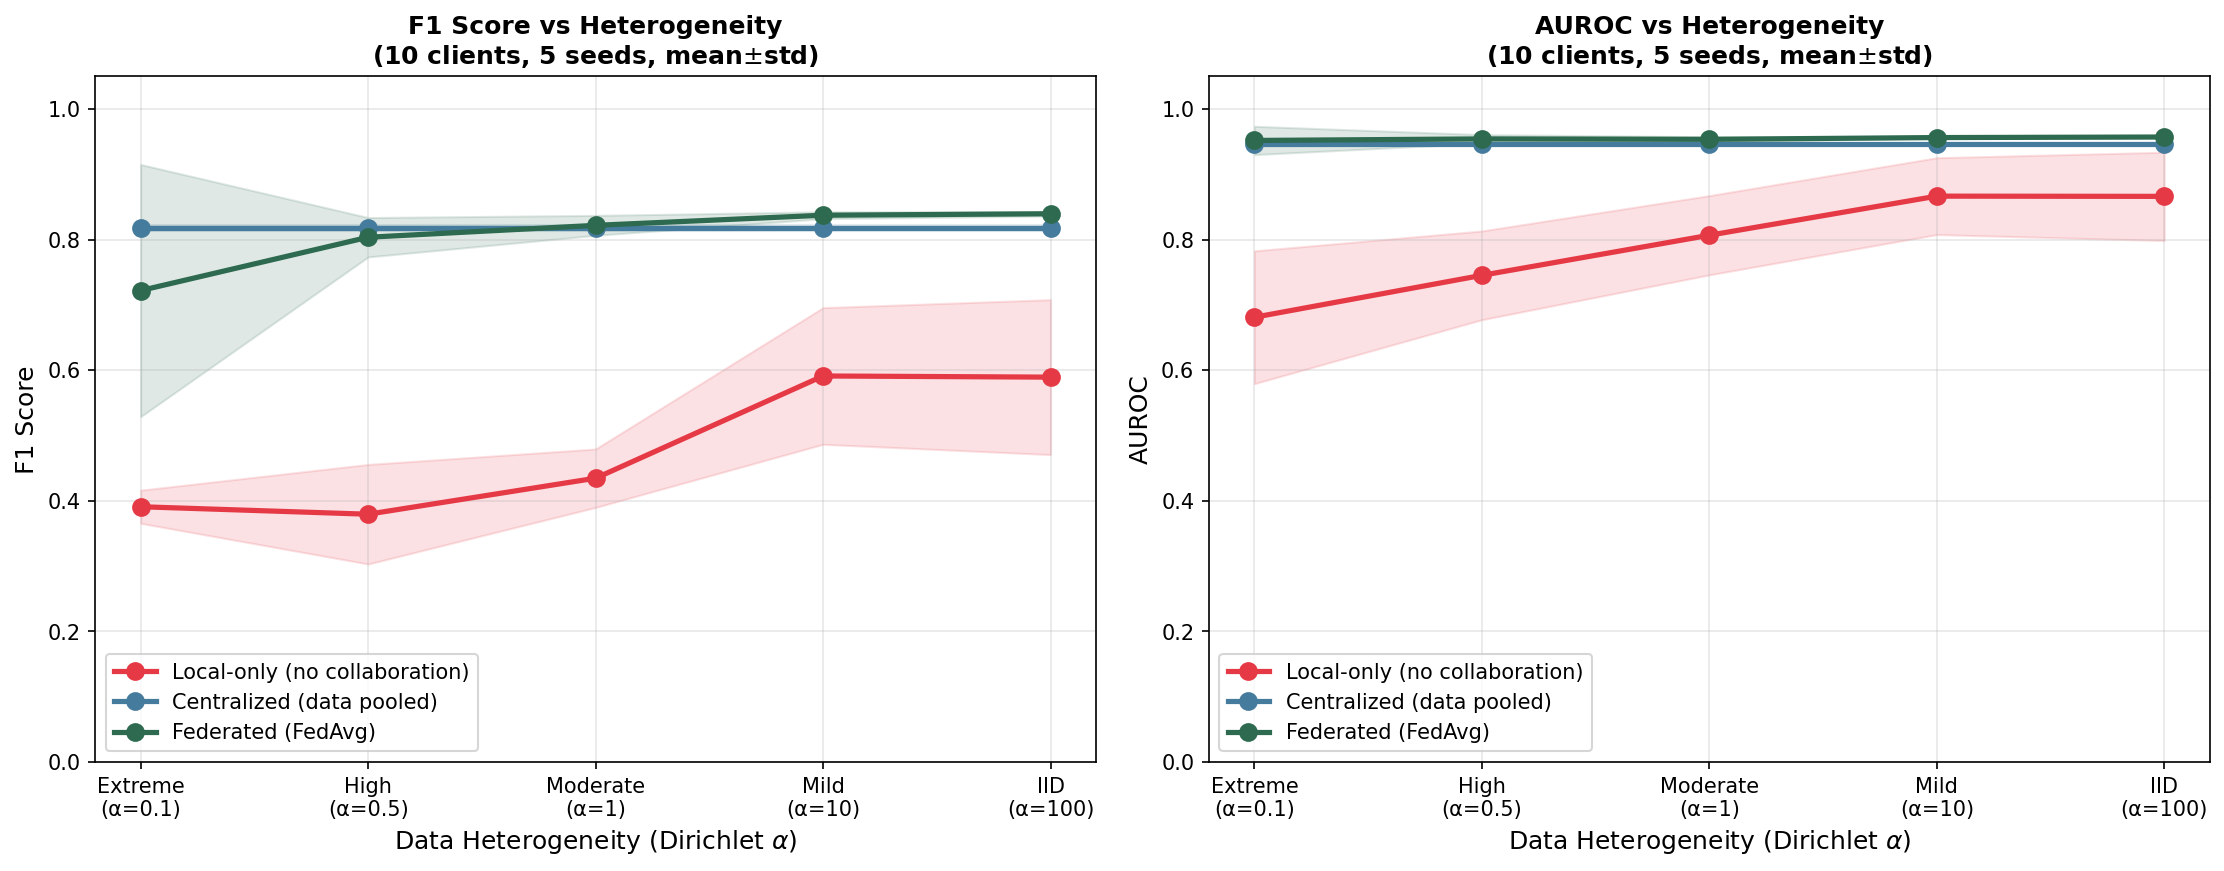
\includegraphics[width=0.95\colwidth]{results/heterogeneity_sweep.png}
    \end{figure}
    {\footnotesize Fig.\,4. At $K$=10 clients, federation \textit{wins}
    across IID to moderate heterogeneity (F1 0.84 vs.\ 0.82 centralized),
    consistent with the isolation study: above the critical client-count
    threshold, FedAvg works as expected.}
  \end{block}

  \begin{block}{Discussion}
    \small
    \begin{figure}
      \centering
      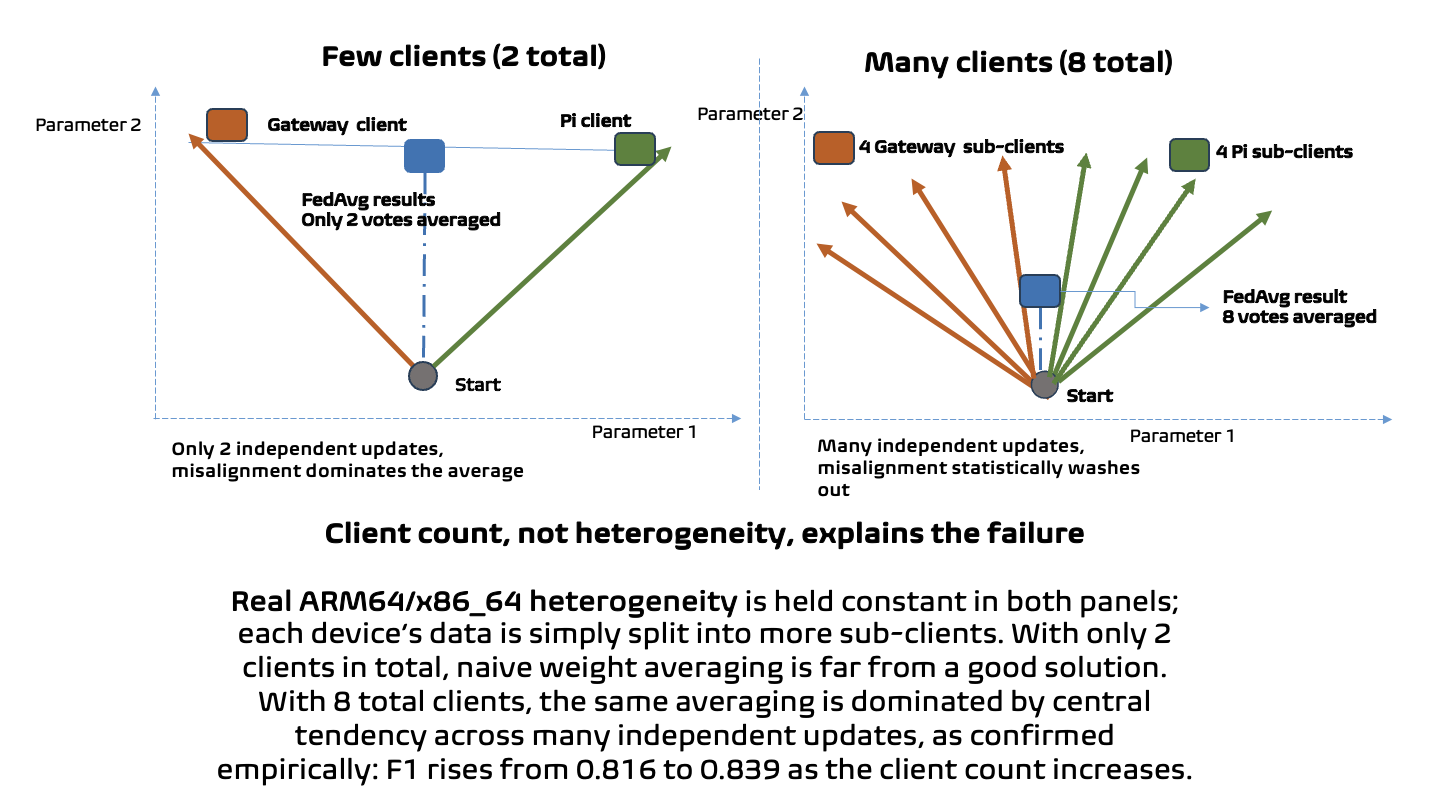
\includegraphics[width=0.95\colwidth]{results/client_count_diagram.png}
    \end{figure}
    {\footnotesize Fig.\,5. Weight-space misalignment: with 2 clients,
    naive averaging lands far from both optima. With 8 clients, updates
    average toward a stable central solution.}

    \vspace{0.15em}
    Two independently trained neural networks solving the same task may
    arrive at very different weight configurations. FedAvg averages these
    directly -- frequently violated between just two networks, producing a
    result resembling neither original solution. With more clients,
    misalignment statistically washes out, exactly the pattern the
    isolation experiment demonstrates.

    \vspace{0.15em}
    \textbf{Practical implication:} for a small pilot fleet (2--5 devices),
    test local-only and centralized pooling as baselines before committing
    to FedAvg. If privacy prohibits pooling, split each device's data into
    virtual sub-clients within FedAvg -- our isolation study shows this
    recovers much of the accuracy loss without adding physical hardware.
  \end{block}

  \begin{block}{Conclusion}
    \small
    Naive FedAvg substantially underperforms both alternatives on a minimal
    2-device real edge deployment -- confirmed across 3 seeds with matched
    training budgets. A controlled isolation experiment demonstrates
    conclusively that \textbf{client count, not heterogeneity, is the
    causal variable}. \textbf{Practitioners should not assume FedAvg is
    unconditionally beneficial on small edge fleets}: at 2--3 clients,
    it can actively underperform simpler alternatives.
  \end{block}

  \begin{block}{Limitations}
    \small
    \begin{itemize}\setlength\itemsep{0.05em}
      \item Only 2 physical devices; sub-clients are data partitions,
            not genuinely independent hardware.
      \item FedProx~\cite{fedprox} and SCAFFOLD~\cite{scaffold}
            not yet tested as remedies at the 2-client scale.
      \item Single task domain; generalization to image/video tasks
            not yet evaluated.
      \item Energy consumption and unreliable networks not yet measured.
    \end{itemize}
  \end{block}

  \begin{block}{References}
    \scriptsize
    \begin{thebibliography}{9}
    \bibitem{fedavg} McMahan et al. (2017). Communication-Efficient Learning
    of Deep Networks from Decentralized Data. \textit{AISTATS}.
    \bibitem{hsu} Hsu et al. (2019). Measuring the Effects of Non-Identical
    Data Distribution for Federated Visual Classification. \textit{arXiv:1909.06335}.
    \bibitem{fedprox} Li et al. (2020). Federated Optimization in
    Heterogeneous Networks. \textit{MLSys}.
    \bibitem{scaffold} Karimireddy et al. (2020). SCAFFOLD: Stochastic
    Controlled Averaging for FL. \textit{ICML}.
    \bibitem{fediot} He et al. (2021). Federated Learning for IoT:
    On-Device Anomaly Detection. \textit{arXiv:2106.07976}.
    \bibitem{tinyfl} Marfo et al. (2025). A Framework for Tiny FL in
    Resource-Constrained IIoT Environments. \textit{IEEE}.
    \bibitem{marconi} Farooq et al. (2024). Harnessing FL for Anomaly
    Detection in Supercomputer Nodes. \textit{FGCS}, 161, 673--685.
    \bibitem{smartgrid} Labate et al. (2026). Towards Secure and Scalable
    Energy Theft Detection. \textit{arXiv:2602.16181}.
    \end{thebibliography}
  \end{block}

\end{column}
\separatorcolumn
\end{columns}
\end{frame}
\end{document}
